\chapter{Conclusion, discussion and prospect}
The $\it{CP}$ parameters measurement is performed based on the validation of analysis strategies by blind analysis.  
In the MC study, the fit is performed which shows a consistent result for $\it{CP}$ parameters compared to the simulation input. The linearity and pull of the $\it{CP}$ fit are checked to validate the reliability of the fit procedures. The fit result on $B^0$ lifetime using experiment data is also agreed with the current value in PDG with a relatively large statistical uncertainty due to the low statistics from data.

After the $\it{CP}$ fit procedures are validated, the $\it{CP}$ parameters $\mathcal{S}$ and $\mathcal{A}$ using Belle II early data with 62.8 ab$^{-1}$in 2019 and 2020 spring and summer is performed. The result is shown in Equation \ref{eq:data_fit_cp}.

\begin{equation}\label{eq:data_fit_cp}
\begin{split}
\mathcal{S}=- sin(2\phi_1) & = -0.82 \pm 0.85(\text{stat}) \pm 0.07(\text{syst}) \\
\mathcal{A} & = -0.21\pm 0.28(\text{stat}) \pm 0.06(\text{syst})\\
\end{split}
\end{equation}  

The result agrees with the prediction of the Standard Model and the previous results from Belle and BaBar. The systematics study is performed considering the main contributing sources at the moment. The measurement precision of $\it{CP}$ parameters in this study is majorly limited due to the large statistical uncertainties from low statistics, which leads to no clear evidence or hint on the NP effects. 
 
In this thesis, the analysis strategies that aim to maximize the efficiency and purity are developed and a conservative measurement approach is taken for the Belle II early data. The newly developed \textit{KsFinder} contributes much in improving the signal significance by effectively rejecting fake $K_S^0$, which is also useful in background rejection for other channels with $K_S^0$ in the final state.  The model of the resolution of vertex positions has been studied using MC sample and sideband data, which is benefiting from the understanding of vertex reconstruction performance in the current Belle II detectors. To make a proper use of the reconstructed vertex information and perform $\it{CP}$ fit compactly, a new $\it{CP}$ fitter is built and being validated, which will serve as a multi-functional analysis tool for Belle II $\it{CP}$ violation study in future. 
 
 %The Belle II experiment is crucial in these channels because of the cleaner background environment and better sensitivity compared with LHCb.

\section{Improvements on statistical uncertainty}
This study has shown a good potential of performing $\it{CP}$ measurement in Belle II for the incoming years with more data recorded. The precision on $\mathcal{S}$ requires the large luminosity as shown in Figure \ref{fig:sensitivity} and the statistical uncertainty in this thesis fits in the scale. With 50 $ab^{-1}$ luminosity from the full Belle II data sample in future, the statistical uncertainty is expected to be reduced. The $\it{CP}$ fit on the MC sample with different mount of events used reflects that the statistical uncertainty is reduced proportionally around factor of $\frac{1}{\sqrt{N}}$, where $N$ is the events used in $\it{CP}$ fit. Also, due to the flavor tagging accuracy limitation, the expected statistics of tagged events could be increased as well, however, at this moment no clear sign of large boosting on flavor tagging efficiency or reduction of wrong tagging fraction is foreseen. Therefore, the expected reduction of statistical uncertainty is mostly due to the increased data sample, with current reconstruction efficiency assumed, which is shown in Figure \ref{fig:stats_future}.  As the current luminosity is quite far away from 50 ab$^{-1}$, it is hard to precisely predict the uncertainty in full Belle II luminosity. Given that the expected sensitivity of $\Delta S$ is in a precision level of $\sim 0.001$, therefore such a precision is taken to estimate the future uncertainties based on the current results. The estimated statistical uncertainty is  $\sim 0.030$ as shown in Figure \ref{fig:stats_future}, which is slightly improved compared to the original estimation at 0.037 from Belle II technical design report in Table \ref{tab:sensitivity}. 

From Table \ref{tab:b0stats}, the current $B^0$ reconstruction efficiency is about 35\% which could be further optimized mainly by improving $K_S^0$ efficiency. As discussed in chapter 3, the $K_S^0$ reconstruction efficiency and quality becomes worse for long-flight ones. This is mainly due to the limitation of CDC-only tracking and the hit filters on the SVD layers. The current Belle II track finding algorithm rises a requirement for SVD hits that at least two or more SVD hits are considered from a same track so that they can be used together with CDC tracks. If a $K_S^0$ decay outside of layer 5 at 10.4 cm, even though the daughter tracks pass the SVD layer 6, unless they hit the overlapping region of the SVD edges, otherwise the tracks are fitted with only CDC hits. This effect is shown in Figure \ref{fig:svd-r-xx}, where \textit{SVD00} type $K_S^0$ start to appear at SVD layer 5. Such a algorithm is to suppress the beam background and SVD noise strips that create a large fraction of random single hits. Thus, the actual sensitivity volume of SVD is reduced and the $K_S^0$ efficiency is negatively affected. 
In future, the improvement of tracking algorithm is expected to remove this requirement while still be able to effectively reduce single hits background.

\begin{figure}[htpb]
	\centering
	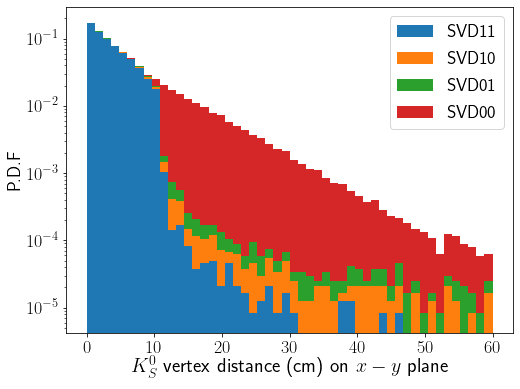
\includegraphics[width=0.7\linewidth]{ks-r-svdxx}
	\caption{$K_S^0$ flight length on $x-y$ plane for each category of $K_S^0$, where \textit{SVD00} type $K_S^0$ start to appear at about SVD layer 5.}
	\label{fig:svd-r-xx}
\end{figure}




In general, the expected $B^0$ signal yield can be improved in future and help to further reduce the statistical uncertainty. From Figure \ref{fig:stats_future}, the projected statistical uncertainty at $0.711$ ab$^{-1}$ using current value is comparable with the Belle result. 
When the integrated luminosity reaches about 9 ab$^{-1}$, the statistical uncertainty is reduced to $\sim 0.072$ which is equivalent to the current systematic uncertainty. At 50 ab$^{-1}$ integrated luminosity, the major contribution will be systematic uncertainty if no improvement is assumed. We take the extrapolated statistical uncertainty $\sim 0.030$ at 50 ab$^{-1}$ as a conservative value for estimating total uncertainty later.

\begin{figure}[htpb]
\centering
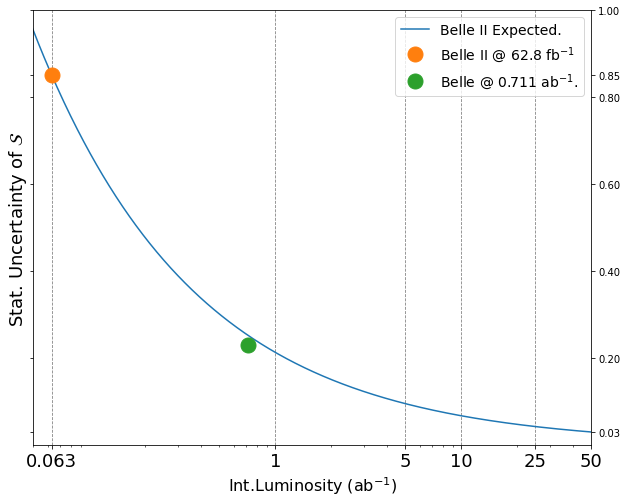
\includegraphics[width=0.7\linewidth]{stats_b2}
\caption{Statistical uncertainty of $\mathcal{S}$ extrapolation based on the current result of $B^0 \to K_S^0  K_S^0  K_S^0$ in Belle II, where the orange is the current value and the green is the Belle result at 0.711 ab$^{-1}$ $\Upsilon$(4S) data.}
\label{fig:stats_future}
\end{figure}

\section{Improvements on systematic uncertainty}
As discussed in the introduction chapter, the NP effects that potentially contributes to the $B^0\to \phi K_S^0$ could also affect $B^0 \to K_S^0  K_S^0  K_S^0$. In the current SM correction, the QCD factorization (QCDF) scan approach suggests the expected upper-limit for $\Delta \mathcal{S}$ is about 0.05\cite{b2book}, and the ``add-in-quadrature" QCDF predicts the $\Delta S = 0.01 \sim 0.02$\cite{b2book}. In this scale, it's important to evaluate the reducible and irreducible systematic uncertainties in $B^0 \to K_S^0  K_S^0  K_S^0$ for future data collection based on the current measurement result. 
%QCDF generally predicts definite or preferred signs of the $\Delta \mathcal{S}$ shift, which implies a definite pattern of shifts to be compared with data\cite{b2book}. At present thereis no significant tension between these predictions and data. 
The irreducible sources mainly refer to the terms that are not scaled or improved with increased luminosity, such as the irreducible vertexing related terms and tag-side interference. The reducible sources are mainly signal $\Delta t$ shape , signal fraction, background $\Delta t$ shape, flavor tagging, and fit bias. As an initial study in early operation with very low statistics, it's summed that the reducible terms are achieved from the increased future luminosity where the reduction of parameters' uncertainties are scaled by the fraction of squared-root of increased events statistically. If no improvement on systematic uncertainty is expected from the current evaluation, with full Belle II data it is still challenging to validate the evidence of the NP effects against the small theoretical predictions. In the Belle II original prospect, the new PXD detector would be contributive to the reduction of vertexing related systematic uncertainties on the average factor of two\cite{b2book}, yet concerning that PXD is not yet fully installed at present and the current vertex reconstruction doesn't include IP constraint options, the conservative scenario that systematic uncertainties do not change due to the largely improved vertexing quality is assumed, which makes the increased luminosity the major factor for precision improvements. To show the estimated systematic uncertainties in future, the data collection as well as MC simulation at 50 ab$^{-1}$ is taken as reference. Similar to the discussion in statistical uncertainties, the precision level of the estimation is set to $\sim 0.001$.

For signal $\Delta t$ shape, we assumed that the $\it{CP}$-side resolution functions parameters can optimized by increased \textit{signal MC} and better vertex reconstruction. The overall 50\% reduction in the uncertainties of $\it{CP}$ side resolution parameters is assumed. The tag-side parameters are determined from 2 ab$^{-1}$ control sample MC which could be further reduced at Belle II  50 ab$^{-1}$ luminosity so the reduced uncertainties are expected to be about 20\% of the current ones. In Table  \ref{tab:sig_shape}, the improvement where both $\it{CP}$ and tag side uncertainties are reduced is calculated while a conservative case that $\it{CP}$ side resolution remain as the present ones is also considered.
\begin{table}[H]
		\centering
		\caption{ Signal $\Delta t$ shape systematic uncertainties of $\mathcal{S}$ expected at 50 ab$^{-1}$. The second and third columns are the expected reduced systematic uncertainties for both $\it{CP}$/tag-side improvements or only tag-side improvement.}
		\label{tab:sig_shape}
		\begin{tabular}{c| c| c }
			\hline
			Luminosity (50 ab$^{-1}$) & both ($\it{CP}$/tag) improved & only tag-side improved \\
			\hline
			signal $\Delta t$ shape &  $\sim0.015$ & $\sim0.030$\\
			\hline
		\end{tabular}
\end{table}
For the signal fraction contribution which is the largest term in the systematic uncertainties currently, it mainly suffers from the very low statistics in data that causes the inaccurate description of signal shape against background. The signal fraction is determined event-by-event using $M_{bc}$ and $\Delta E$ 2D fit shape in Figure \ref{fig:2Ddata}. Hence, the uncertainties of signal fraction parameters are expected to be reduced quickly with the increased data collection in future. Using 1 ab$^{-1}$ \textit{generic MC}, the signal fraction contribution is estimated for comparison, where the combined contribution on $\mathcal{S}$ uncertainty by floating $\pm 1 \sigma$ for each parameter is $\sim 0.013$. This estimation is close to the observed systematic uncertainty from signal fraction in  Belle data which is  $\sim0.015$\cite{kang2020measurement} and the data scaled value  $\sim 0.011$, both with $\mathcal{O}(0.01)$ level difference. Therefore, the current contribution is taken as the baseline to extrapolate the reduced systematic uncertainty in 50 ab$^{-1}$ Belle II data, reduced by luminosity ratio to $\sim 0.002$, listed in Table \ref{tab:sig_f}.

\begin{table}[htpb]
	\centering
	\caption{ Signal fraction systematic uncertainties of $\mathcal{S}$ expected at 50 ab$^{-1}$.}
	\label{tab:sig_f}
	\begin{tabular}{c| c}
		\hline
		Luminosity (50 ab$^{-1}$) & Improved uncertainty \\
		\hline
		Signal fraction &  $\sim0.002$ \\
		\hline
	\end{tabular}
\end{table}

For the background $\Delta t$ shape, it can be reduced by the increased luminosity since the current parameters are determined by sideband data with very low statistics. Therefore, the systematic uncertainty from background $\Delta t$ shape is reduced by factor $\sim 28$ calculated from $\sqrt{50/0.063}$ to be $\sim 0.001$ as listed in Table \ref{tab:bkg_shape}. This estimation is checked by comparing the background $\Delta t$ shape uncertainties in between Belle result and the one in this analysis, where the background $\Delta t$ shape contribution in Belle is 0.017\cite{kang2020measurement} with a tighter sideband region used, which is consistent with scaled luminosity of Belle. 

\begin{table}[htpb]
	\centering
	\caption{ Background $\Delta t$ shape systematic uncertainties of $\mathcal{S}$ expected at 50 ab$^{-1}$.}
	\label{tab:bkg_shape}
	\begin{tabular}{c| c}
		\hline
		Luminosity (50 ab$^{-1}$) & Improved uncertainty \\
		\hline
		Background $\Delta t$ shape &  $\sim0.001$ \\
		\hline
	\end{tabular}
\end{table}

For the contributions of wrong tag fraction, the flavor tagging related information is expected to be determined by experimental data using flavor-specific decay modes with increased Belle II data in future. To estimate the expected uncertainties from Belle II future data, the results on $w$ in each $r$-bin by using about 8.7 fb$^{-1}$ Belle II in 2019 are compared with the Belle results\cite{abudinen2020first}. The flavor tagging performance studied by Belle II early data presented a close efficiency and wrong tag fraction values compared to Belle results. In each $r$-bin, the uncertainties of $w$ is reduced averagely by factor of $\sim 11$, which is consistent with the squared root of the luminosity ratio. Hence, the expected uncertainties at 50 ab$^{-1}$ Belle II data is assumed to be $\sim 7$ times smaller than those from the Belle result\cite{kang2020measurement}, which is about $\sim0.002$ as listed in Table \ref{tab:wtag_50ab}.

\begin{table}[htpb]
	\centering
	\caption{ Wrong tag fraction systematic uncertainties of $\mathcal{S}$ expected at 50 ab$^{-1}$.}
	\label{tab:wtag_50ab}
	\begin{tabular}{c| c}
		\hline
		Luminosity (50 ab$^{-1}$) & Improved uncertainty \\
		\hline
		wrong tag fraction &  $0.002$\\
		\hline
	\end{tabular}
\end{table}

For the fit bias contribution as systematic uncertainty, currently the values are taken by the statistical fit error using 300000 \textit{signal MC}. In future, the fit bias contribution is expected to be estimated by taking the larger one among the fit statistical error using more MC sample and the center value difference between the input and output. Thus, if MC sample used in fit could be at least 100 times more than one million in future, then the fit error is possible to be smaller than input-output difference. From the current MC production plan of Belle II, the  \textit{signal MC} sample recommended by MC production group is typically in a range of several millions. So the foreseen systematic uncertainty is still going to be the fit error, where we take a 50\% reduction as an estimation similar to the one used in $\it{CP}$-side resolution functions, listed in Table \ref{tab:fitbias_full}.

\begin{table}[htpb]
	\centering
	\caption{ Fit bias systematic uncertainties of $\mathcal{S}$ expected at 50 ab$^{-1}$.}
	\label{tab:fitbias_full}
	\begin{tabular}{c| c}
		\hline
		Luminosity (50 ab$^{-1}$) & Improved uncertainty \\
		\hline
		fit bias &  $\sim 0.005$ \\
		\hline
	\end{tabular}
\end{table}

Concluded from the above discussion, the reducible systematic uncertainties by using increased MC and data in full Belle II luminosity are estimated and summarized in Table \ref{tab:reducedsys}. It is clear that the dominated contribution in future Belle II data for systematic uncertainty is the $\it{CP}$ side resolution, indicating the finer study on $\it{CP}$ side resolution model for no IP-originated tracks is necessary with much larger data sample.
In addition, the impact of using \textit{KsFinder} receives contribution from the data MC mismatch on signal purity, which is expected to be improved by better data MC consistency in future. For physics parameters $\Delta m_d$ and $\tau_{B^0}$, the uncertainties could be further reduced by better physics input. Finally, vertex reconstruction options are not contributing much in this analysis mostly because of the very loose cuts and no IP constraint used. However, this does not mean their contributions are missing since the resolution function parameters obtained under such loose IP conditions receives more inaccuracies than the ones from using tighter cuts and IP constraint. The signal $\Delta t$ shape contribution partially absorbs the expected uncertainties from vertex reconstruction options. In future, by using proper IP constraint and tighter vertex cuts, the signal $\Delta t$ shape will contribute less and vertex reconstruction will contribute more to systematic uncertainties. We keep the current estimation from \textit{KsFinder}, physics parameters and the vertex reconstruction as the ones in 50 ab$^{-1}$ Belle II luminosity to have a conservative expectation on $\mathcal{S}$ systematic uncertainty.

\begin{table}[htpb]
	\centering
	\caption{ Improved systematic uncertainties of $\mathcal{S}$ expected at 50 ab$^{-1}$. The value in the parenthesis stands for the case that only tag-side resolution is improved and no improvement on $\it{CP}$ side resolution is implemented. }
	\label{tab:reducedsys}
	\begin{tabular}{c| c}
		\hline
		Sources & Improved uncertainty (50 ab$^{-1}$) \\
		\hline
		signal $\Delta t$ shape &  $\sim$0.015($\sim$0.030)\\
		Signal fraction &  $\sim$0.002 \\
		Background $\Delta t$ shape &  $\sim0.001$\\
		wrong tag fraction &  $\sim0.002$\\
		fit bias &  $\sim0.005$\\
		\hline
	\end{tabular}
\end{table}


\section{Total uncertainty of $\Delta S$ at 50 ab$^{-1}$}
The total systematic uncertainty of $\mathcal{S}$ in 50 ab$^{-1}$ Belle II luminosity is estimated based on the improved terms and the unchanged ones. If $\it{CP}$ side resolution is not improved, the systematic uncertainty is $\sim$0.031. If the $\it{CP}$ side resolution functions is 50\% improved, the systematic uncertainty is reduced to  $\sim0.016$. Both are shown in Table \ref{tab:sys_full} where the major contribution is from signal $\Delta t$ shapes which is related to the vertexing quality. 

\begin{table}[htpb]
	\centering
	\caption{The systematic uncertainty expected in 50 ab$^{-1}$ Belle II luminosity. The first column is the current value of systematic uncertainty of $\mathcal{S}$ in $B^0 \to K_S^0  K_S^0  K_S^0$. The second and third columns are the systematic uncertainties for both $\it{CP}$/tag-side improvements or only tag-side improvement used in the combined estimation.}
	\label{tab:sys_full}
	\begin{tabular}{c| c | c |c}
		\hline
		Luminosity(ab$^{-1}$) & current($\sim$0.063) & $\it{CP}$/tag(50)& only-tag(50)\\
		\hline
		Syst.Uncert.($\mathcal{S}$) & $\sim0.072$ & $\sim$0.016 & $\sim0.031$\\
		\hline
	\end{tabular}
\end{table}


By adding in quadrature using estimated statistical and systematic uncertainties, the total uncertainty for $\mathcal{S}$ in $B^0 \to K_S^0  K_S^0  K_S^0$ in 50 ab$^{-1}$ Belle II luminosity is estimated, as shown in Table \ref{tab:err_full}. With no $\it{CP}$ vertex resolution improvement, total uncertainty of $\sim 0.043$ is expected. On the other hand, the total uncertainty will be at $\sim 0.034$ if 50\% $\it{CP}$-side resolution improvement is assumed, which is a achievable considering that the current $\it{CP}$-side vertexing performance is not optimized yet. In this case, the statistical uncertainty even at 50 ab$^{-1}$ luminosity is still the major contribution. Given the total uncertainty from $B^0\to J/\psi K_S^0$ at that time is expected to be $\sim 0.005$\cite{b2book}, $\Delta S$ sensitivity is dominated by the total uncertainty in $B^0 \to K_S^0  K_S^0  K_S^0$. The current Belle result from $B^0 \to K_S^0  K_S^0  K_S^0$ on $\Delta S$ is $\sim0.05$ without taking into account any uncertainty, which is close to the theoretical predicted upper-limit. In general, a total uncertainty at about $0.034\sim 0.043$ for $\Delta S$ at Belle II full luminosity is expected to be a much better probe for addressing whether the NP effects in $B^0 \to K_S^0  K_S^0  K_S^0$ exist.

\begin{table}[htpb]
	\centering
	\caption{The total uncertainty of $\mathcal{S}$ in $B^0 \to K_S^0  K_S^0  K_S^0$ expected in 50 ab$^{-1}$ Belle II luminosity, calculated from the expected statistical and systematic uncertainties. The second and third columns are the total uncertainties for both $\it{CP}$/tag-side improvements or only tag-side improvement used in the combined estimation.}
	\label{tab:err_full}
	\begin{tabular}{c|c|c |c}
		\hline
		Luminosity (ab$^{-1}$) & current($\sim$0.063)&$\it{CP}$/tag(50) & only-tag(50)\\
		\hline
		Tot.Ucert.($\mathcal{S}$) & $\sim0.853$ & $\sim0.034$ & $\sim0.043$ \\
		\hline
	\end{tabular}
\end{table}

\section{\textit{KsFinder} importance}
While monitoring the uncertainties of the $\it{CP}$ parameters is crucial in searching the hidden NP effects, avoiding bias in the measurement is also critical. If a total uncertainty at $\sim 0.03$ is achieved in future, however, the center value of $\mathcal{S}_{3K_S^0}$ is biased and shifted away from $\mathcal{S}_{J/\psi K_S^0}$, it can lead to a very wrong conclusion about the discovery of the NP effects.
The \textit{KsFinder} contributes to improve the signal purity for measuring $\it{CP}$ parameters, which is essential in controlling the potential bias introduced by the large fraction of background events that yield random $\it{CP}$ asymmetry due to the statistical fluctuation. The larger background events without using \textit{KsFinder} cut in Table \ref{tab:b0select} can produce the wrongly estimated signal fraction ($f_{sig}$) in Equation \ref{eq:tdcpv_all_res} so that the $\it{CP}$ parameters are biased using the biased fit model. Especially when the luminosity is increased in future, the signal fraction uncertainty is expected to be largely reduced, such a biased signal fraction will be treated as a large contribution to the systematic uncertainty compared to the correct ones. 
To demonstrate the effect,  the signal extraction and $\it{CP}$ fit on the 1 ab$^{-1}$ \textit{generic MC} sample without \textit{KsFinder} are performed. In this case, we remove the \textit{KsFinder} cut in Table \ref{tab:b0select} and apply the cut $cosVertexMomentum > 0.9$ which can only achieve $\sim 82\%$ purity for $K_S^0$ in \textit{signal MC}. The signal significance in $M_{bc}$ and $\Delta E$ 2D fit is considerately lower than the ones with using \textit{KsFinder}. The stacked histograms of $M_{bc}$ and $\Delta E$ with much higer background are shown in Figure \ref{fig:hist_2D_highBG} where the red component is signal. There are 352 true signal events and 543 background events inside the signal region by count. In the meanwhile, the 2D fit on $M_{bc}$ and $\Delta E$ are shown in Figure \ref{fig:2Ddata_noks}. From the 2D fit, the signal events number is $389\pm19$ and background events number is $502\pm15$. Clearly the signal fraction defined by the 2D fit in the latter case is biased from the MC truth, which shows a positively biased signal fraction on average, as summarized in Table \ref{tab:ksbias}.

\begin{table}[htpb]
	\centering
	\caption{The signal and background events using different $K_S^0$ selection cuts compared with the \textit{generic MC} counts, showing that signal events reconstructed using \textit{KsFinder} is more precise to the MC truth. }
	\label{tab:ksbias}
	\begin{tabular}{c| c |c}
		\hline
		Selection & signal  & background \\
		${FBDT\_Ks>0.74}$ (fit) & $341\pm20$ & $61\pm17$ \\
		${FBDT\_Ks>0.74}$ (MC) & 336 & 68\\
		${cosVertexMomentum>0.9}$ (fit) & $389\pm19$ & $502\pm15$\\
		${cosVertexMomentum>0.9}$ (MC) & 352 & 543\\
		\hline
	\end{tabular}
\end{table}

From Table \ref{tab:ksbias}, by using \textit{KsFinder}, the true average signal fraction in signal region from 1 ab$^{-1}$ \textit{generic MC} is 83.2\%, and the fit result is $(84.8\pm3.7)\%$. To contrary, by only using ${cosVertexMomentum>0.9}$, the true average signal fraction is 39.3\% and the fit result is $(43.7\pm1.4)\%$, which shows over $3\sigma$ deviation as a strong bias. If such a bias is taken into account as the systematic uncertainty, signal fraction difference is used as a floating value to check the impact on the $\it{CP}$ fit results, which leads to an extra systematic uncertainty from the biased $f_{sig}$ at level of $\sim 0.006$, already larger than any other source except for the signal $\Delta t$ shapes as listed in Table \ref{tab:sys_full}. Therefore, the development of \textit{KsFinder} is particularly important in the precised $\it{CP}$ measurement for $B^0 \to K_S^0  K_S^0  K_S^0$. The current performance of \textit{KsFinder} is presenting a purity about 95\% in $K_S^0$ reconstruction which means there is still small room for improvements, as well as the background rejection power. The targeted purity and background rejection power of \textit{KsFinder} in future is $\sim 99\%$ on average. The data/MC consistency should also be improved so the current correction ratio $R_{B^0}$ is expected to be reduced to $\sim 1.00\pm 0.01$. Thus the systematic uncertainty from different \textit{KsFinder} responses in between data and MC is assumed to be $\mathcal{O}(0.001)$ as a negligible contribution. 



\begin{figure}[htbp]
	\begin{minipage}[b]{0.5\linewidth}
		\centering 
		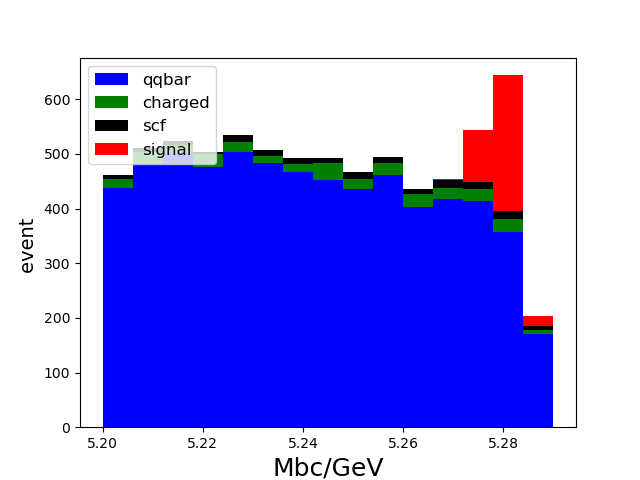
\includegraphics[height=6cm]{figures/hist_stacked_generic_mbc_noksfinder.png}
		\label{}
	\end{minipage}
	\begin{minipage}[b]{0.5\linewidth}
		\centering 
		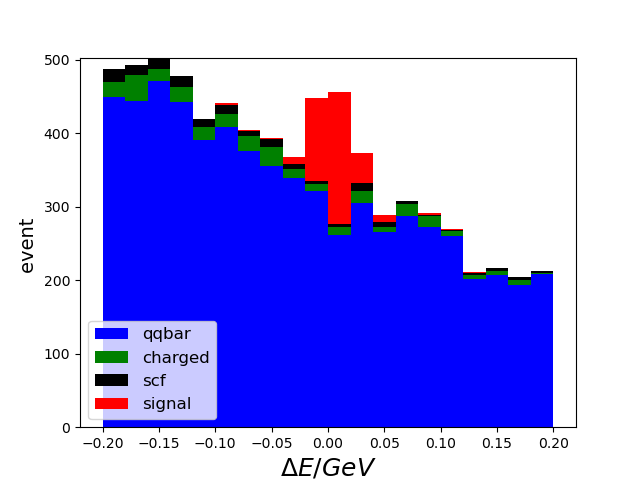
\includegraphics[height=6cm]{figures/hist_stacked_generic_dE_noksfinder.png}
		\label{}
	\end{minipage}
	\caption{$M_{bc}$ and $\Delta E$ stacked histogram of  1 ab$^{-1}$ \textit{generic MC} sample replacing $FBDT\_Ks>0.74$ by ${cosVertexMomentum}>0.9$ in Table \ref{tab:b0select} as a selection criteria, showing a much worse signal significance.}
	\label{fig:hist_2D_highBG}
\end{figure}





\begin{figure}[htbp]
	\begin{minipage}[b]{0.5\linewidth}
		\centering 
		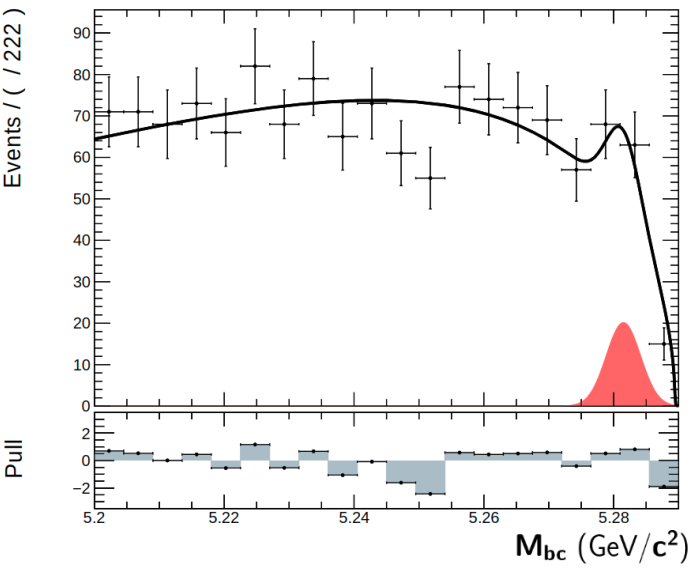
\includegraphics[height=6cm]{figures/mbcfit_noksdata.png}
		\label{}
	\end{minipage}
	\begin{minipage}[b]{0.5\linewidth}
		\centering 
		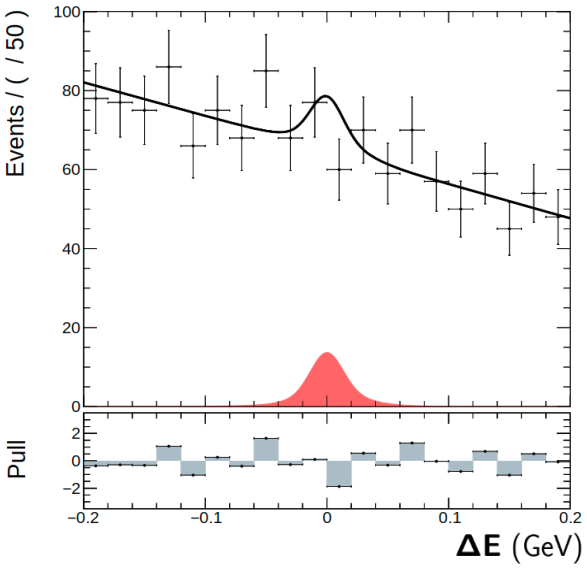
\includegraphics[height=6cm]{figures/dEfit_noksdata.png}
		\label{}
	\end{minipage}
	\caption{$M_{bc}$ and $\Delta E$ 2D fit on 1 ab$^{-1}$ \textit{generic MC} sample, replacing $FBDT\_Ks>0.74$ by ${cosVertexMomentum}>0.9$ in Table \ref{tab:b0select}. The red is signal component.}
	\label{fig:2Ddata_noks}
\end{figure}


\section{Prospect}
Even though the current result on $\it{CP}$ parameters are dominated by the large uncertainty, mostly from the statistical one, the previous discussions about the future uncertainties have shown a good potential of searching for the NP effects in $B^0 \to K_S^0  K_S^0  K_S^0$ based on the current analysis in this thesis. At integral luminosity at 50 ab$^{-1}$, the uncertainty on $\mathcal{S}$ would be reduced to a comparable value around $0.034\sim0.043$ realistically, as shown in Figure \ref{fig:tot_exp}, where the statistical and reducible systematic uncertainties are assumed to be scaled by the squared root of the integrated luminosity. The expected sensitivity in full Belle II data is proven to be competitive and the analysis workflow is built which will be further improved along with the future Belle II data taking and MC production. In conclusion, the progress that has been made so far in this thesis paves a well-constructed and solid path for searching the NP effects in time dependent $\it{CP}$ violation study of $B^0 \to K_S^0  K_S^0  K_S^0$. 
 
\begin{figure}[htpb]
	\centering
	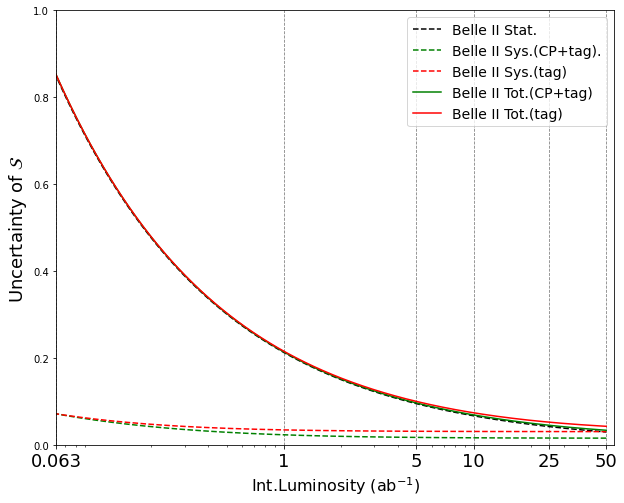
\includegraphics[width=0.7\linewidth]{tot_unc_1}
	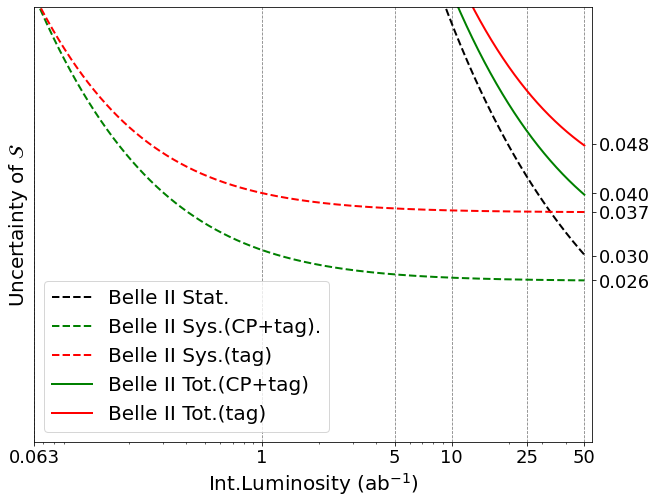
\includegraphics[width=0.7\linewidth]{tot_unc_2}
	\caption{The expected total uncertainty of $\mathcal{S}$ in $B^0 \to K_S^0  K_S^0  K_S^0$, where the dashed lines are the statistical(black), $\it{CP}$/tag-side improved systematic(green) and only tag-side improved systematic(red) uncertainties, with the corresponding solid lines as the total uncertainties. The top is the overview for the whole Belle II luminosity range from now, and the bottom is $y$-axis zoom-in.}
	\label{fig:tot_exp}
\end{figure}

